\documentclass[a4paper,10pt, titlepage]{article}
\usepackage{fullpage}
\usepackage{times}
\usepackage[utf8]{inputenc}
\usepackage{amsmath}
\usepackage{amssymb}
\usepackage{graphicx}
\usepackage{epstopdf}
\usepackage{inputenc}
\usepackage{geometry}
\geometry{left=2.5cm,right=2.5cm,top=2.5cm,bottom=2.5cm}
\usepackage{caption}
\usepackage{subcaption}
\usepackage{times}
\usepackage{graphicx}
\usepackage[font=small,labelfont=bf]{caption}
\usepackage{float}
\usepackage{hyperref}
\usepackage{array}
\usepackage[table]{xcolor}
\AfterEndEnvironment{figure}{\noindent\ignorespaces}

\begin{document}
\font\myfont=cmr12 at 40pt
\font\myfontok=cmr12 at 25pt

\title{%
  \textbf{\myfont AWSS} \\
  \myfontok DNAs substring matching\\
  	\textit{We make biology easier and faster}}

\author{Danilo Modica • Guglielmo Cassini • Alessandro Capici • Domenico Ragusa\\
		\\
		\footnotesize Rev. 1.0 - 05/2022}
\date{}
\maketitle

\clearpage
\tableofcontents

\clearpage
\setcounter{page}{1}

\section{Introduction}
\pagenumbering{arabic}
The purpose of this document is to provide a comprehensive description of the application, outlining its various use cases, behavior in certain situations, requirements met, constraints, and possible future developments.
\subsection{Product purpose}
The web application is designed in order to provide a service for computing matches between two DNA strings. It can be used by a general user who will have the possibility to perform the calculation by connecting directly from his own device to the service website. At that point he will be able to insert two DNA strings and start the calculation. Receiving an email notification afterwards, he can eventually download the result from the same website. 
\section{Requirements}
\subsection{User requirements}
\subsection{System requirements}
\section{System models}
This section will list and illustrate the models that formed the basis of the development of the AWSS web application by showing the scenarios in which a given actor interacts with the system.
\subsection{Use cases}
There are two use cases on which the application is based. These, illustrated in the figure \ref{fig:ucdiag} and described in the tables \ref{tab:uc1d-table} and \ref{tab:uc1b-table} are:
\begin{itemize}
	\item \textbf{UC1D}: Computing the substring
	\item \textbf{UC1B}: On-demand download of previously calculated substrings
\end{itemize}
\begin{figure}[H]
	\centering
	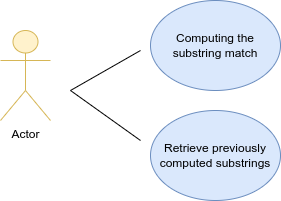
\includegraphics[width=0.4\linewidth]{figures/ucdiag.png}
	\caption{Use cases UML diagram}
	\label{fig:ucdiag}
\end{figure}
\begin{table}
	\centering
\begin{tabular}{ | m{3.5cm} | m{11cm} |}
	\hline
	\rowcolor{lightgray}
	Code & \textbf{UC1D} \\
	\hline
	Name & \textbf{Computing the substring} \\
	\hline
	\rowcolor{lightgray}
	Goal & Starting the calculation of a common substring between two DNA strings\\
	\hline
	Primary actor & Customer \\
	\hline
	\rowcolor{lightgray}
	Stakeholders and interests & \textbf{Customer}: wants to be able to calculate a DNA substring quickly and accurately by entering the DNA strings to be compared. He would like to be notified as soon as the execution of the algorithm is complete.\\
	\hline
	Preconditions & The customer must have a stable internet connection.\\
	\hline
	\rowcolor{lightgray}
	Main success scenario & 
	\begin{itemize}
		\item The client enters the application to begin processing.
		\item The client enters the two starting DNA strings.
		\item The customer specifies the email to which to send notification when finished.
		\item The system loads the files and starts the processing.
	\end{itemize}\\
	\hline
	Special requirements & 
	\begin{itemize}
		\item GUI text must be visible from at least three feet away.
		\item The steps to follow to begin processing should be simple and intuitive.
	\end{itemize}\\
	\rowcolor{lightgray}
	\hline
	Occurence frequency & High, almost continuous\\
	\hline
  \end{tabular}
  \caption{\label{tab:uc1d-table}Description of use case UC1D}
  \end{table}
  \begin{table}
	\centering
\begin{tabular}{ | m{3.5cm} | m{11cm} |}
	\hline
	\rowcolor{lightgray}
	Code & \textbf{UC1B} \\
	\hline
	Name & \textbf{Retrieve previously computed substrings} \\
	\hline
	\rowcolor{lightgray}
	Goal & On-demand download of previously calculated substrings\\
	\hline
	Primary actor & Customer \\
	\rowcolor{lightgray}
	\hline
	Preconditions & A customer has successfully performed a processing.\\
	\hline
	Description & The customer accesses the system and has the ability to download any substring they have previously calculated within the 365-day time limit.\\
	\hline
  \end{tabular}
  \caption{\label{tab:uc1b-table}Description of use case UC1B}
  \end{table}
\subsection{Domain model}
\begin{figure}[H]
	\centering
	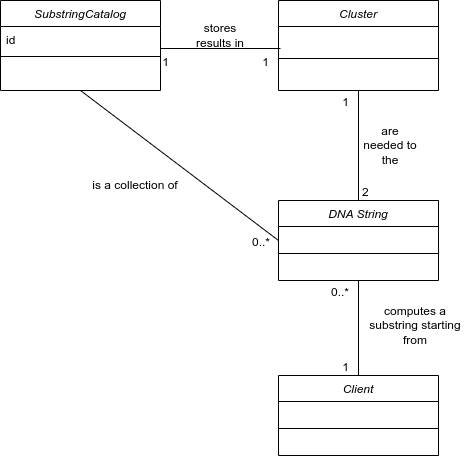
\includegraphics[width=0.5\linewidth]{figures/dommod.png}
	\caption{Domain model}
	\label{fig:dommod}
\end{figure}
%Da spiegare
\section{Architecture}
The high-level architecture is client-server and in particular follows a thin-client model. 
Two different layers can be distinguished:
\begin{itemize}
	\item \textbf{Presentation layer}
	\item \textbf{Data processing and management layer}
\end{itemize}
The management and processing data layer are implemented with the Amazon AWS cloud infrastructure whose architecture is shown in figure \ref{fig:arch}
\begin{figure}[H]
	\centering
	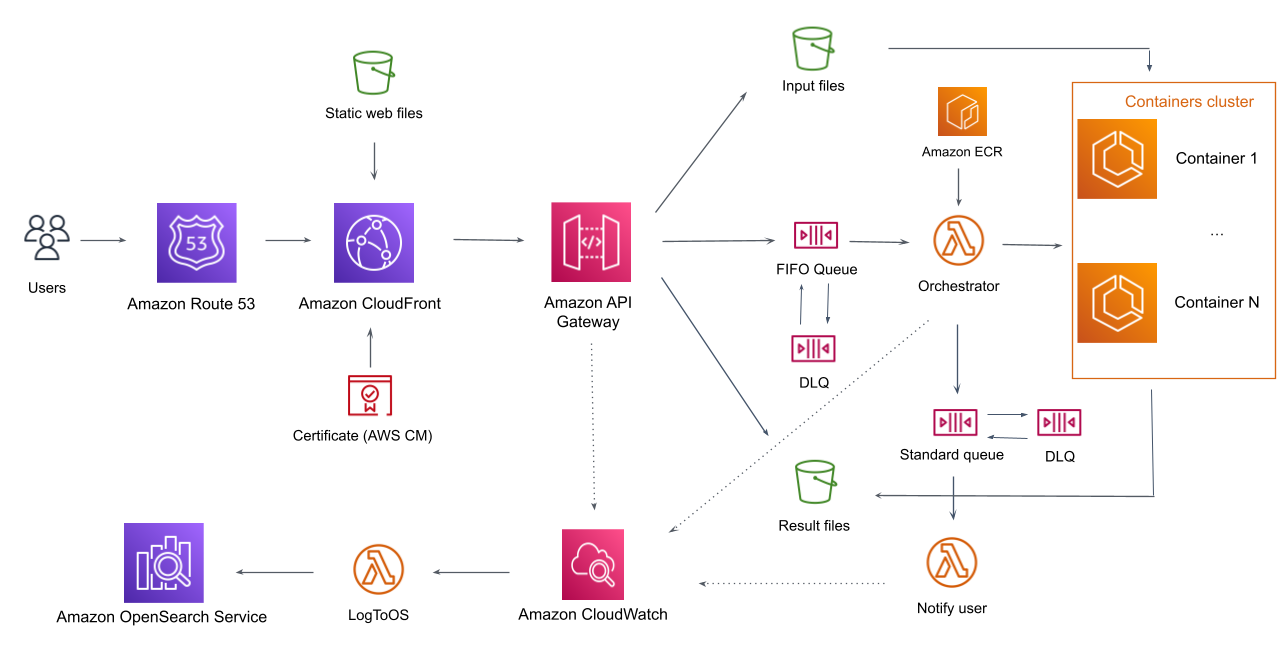
\includegraphics[width=\linewidth]{figures/arch.png}
	\caption{Amazon AWS Architecture}
	\label{fig:arch}
\end{figure}
\section{CI/CD}
\section{Web interface}
The web interface is developed on a single page to improve usability and efficiency in pursuing the user's goal.
In particular, it consists of four sections:
\begin{itemize}
	\item \textbf{Get started}\newline In the first part of the section it is possible to select the two files with the DNA strings to load for processing and to specify the email to which to send a notification in case of success/failure in the processing. In the second part it is possible to insert the code previously sent by email in order to download the result of the associated computation (figure \ref{fig:compute}).
	\begin{figure}[H]
		\centering
		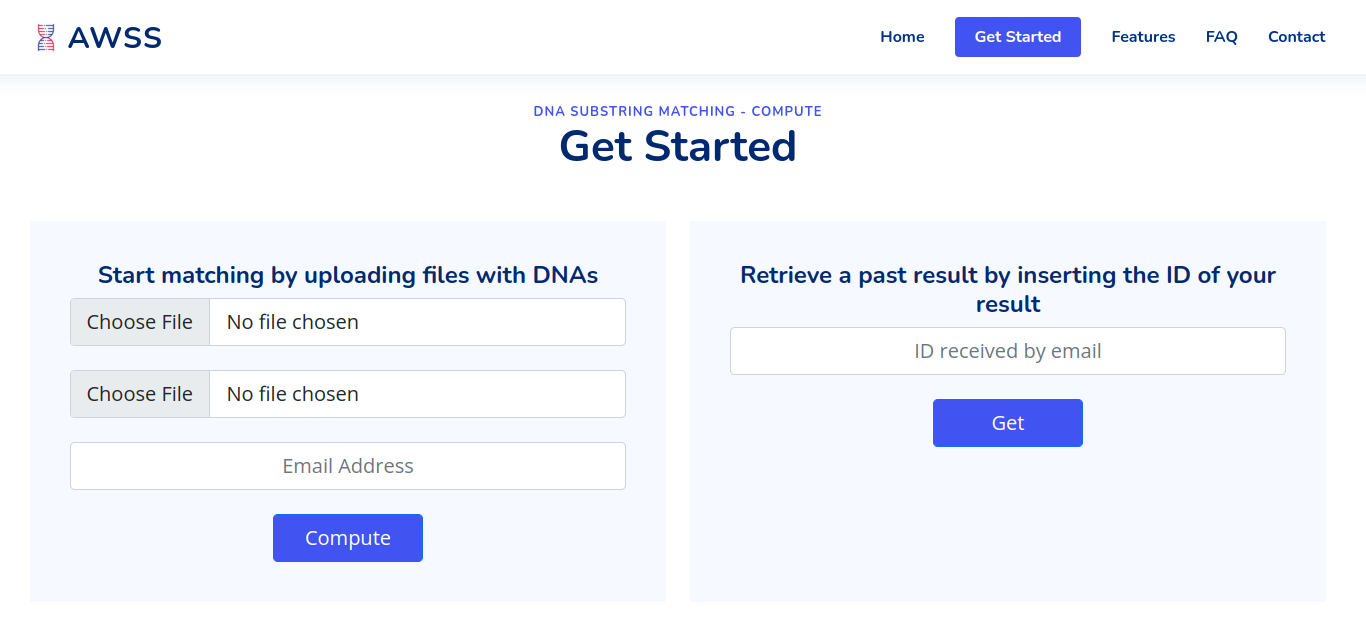
\includegraphics[width=\linewidth]{figures/compute.png}
		\caption{Main section of the interface for interacting with the app}
		\label{fig:compute}
	\end{figure}
	\item \textbf{Features}\newline The main features of AWSS webapp are highlighted
	\item \textbf{FAQ}\newline Section used to clarify the most common doubts of the user with the questions that are often asked (figure \ref{fig:faq}).
	\begin{figure}[H]
		\centering
		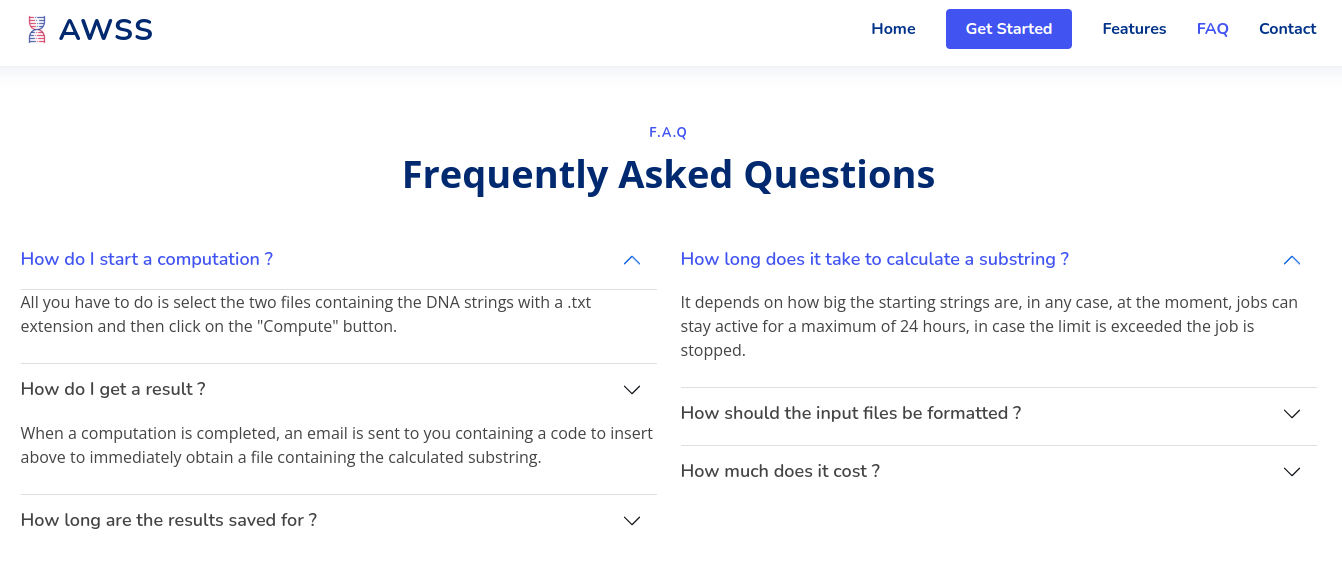
\includegraphics[width=\linewidth]{figures/faq.png}
		\caption{FAQ section of the interface}
		\label{fig:faq}
	\end{figure}
	\item \textbf{Contacts}\newline The contact section contains the main means of contact between the developers and the user in case of problems or to give feedback.
\end{itemize}
\section{Future improvements}
Possible future developments of the application include:
\begin{itemize}
	\item Design of a system for authentication so that the user can easily find all the processes in execution and completed in a restricted area with its results.
	\item Implementation of a system for counting the resources spent in computation and related payment system for authenticated users.
	\item Implement multipart download/upload so that data upload/download is more resilient to network issues and faster due to parallelization.
	\item Modify the algorithm to become distributed so that it can distribute the workload over multiple machines, speeding up data processing.
\end{itemize}
\section{License}
Copyright 2022 AWSS\newline
\newline
Licensed under the Apache License, Version 2.0 (the "License"); you may not use this file except in compliance with the License. You may obtain a copy of the License at\newline
\newline
	http://www.apache.org/licenses/LICENSE-2.0\newline
\newline
Unless required by applicable law or agreed to in writing, software distributed under the License is distributed on an "AS IS" BASIS, WITHOUT WARRANTIES OR CONDITIONS OF ANY KIND, either express or implied.
See the License for the specific language governing permissions and limitations under the License.\newline
\end{document}